\documentclass{article}
\usepackage[utf8]{inputenc}
\usepackage[english,swedish]{babel}

\usepackage{kommfram}
\usepackage{url}
\usepackage{graphicx}

\title{Introduktion till kryptografi och några praktiska användningsområden}
\translatedtitle{Introduction to Cryptography and Some Practical Applications}
\kommedition{Höstterminen 2008}
\kommemail{peterbostrom@gmail.com}
\kommgroup{3}
\kommteacher{Richard Nordberg}
\author{Peter Boström}

\begin{document}

\maketitle
\thispagestyle{empty}
\newpage

\selectlanguage{english}

\begin{abstract}

\noindent This report introduces the reader to cryptography and some of its practical uses. It investigates different methods of concealing information and determines its applications. \\

\noindent The purpose of this report is to investigate and account for some basic principles of cryptography while keeping them as simple as possible. An important part of the report is also cryptanalysis, or rather determining weaknesses in cryptographic systems. The study finds that, while computers used for breaking these systems become significantly faster, some older systems fall short because they were simply not complex enough. \\

\noindent The report also accounts for a few important practical uses of cryptography. It finds areas where the lack of cryptography can have dire consequences. In some of these practical uses, including banking, there's often a secure system built for this purpose. In these areas the user doesn't have to think about security, because the system does that for them. However, there are areas where the user himself have to establish a cryptographic system. By considering these cases the author hopes to establish some basic reflections regarding security. \\

%This article aims to be a start for readers looking for some basic general knowledge on cryptography. The reader will get introduced to some pitfalls and to the importance of cryptography itself, sometimes through examples where it can fail.

%It's neither emphasizing on the math behind cryptography nor how it's actually implemented, but rather where it's used, and why. This way it aims to keep it simple so that anyone not familiar with cryptography can get something out of it.

\end{abstract}

\newpage

\selectlanguage{swedish}

\tableofcontents
\thispagestyle{empty}

\newpage

\setcounter{page}{1}

\section {Vad är kryptografi?}

Kryptografin är en metod för att göra information svårtydbar. Grundidén är att ingen annan än de som är avsedda att ta del av informationen ska kunna göra det. Rövarspråket går att se som en enkel form av kryptering.

Metoder för informationsomvandling kallas för \emph{krypton}. Vid kryptering används en eller flera \emph{nycklar} för att både koda och avkoda informationen.

Relativt enkla krypton för att omvandla text kallas ofta för \emph{chiffer}. Ett enkelt chiffer kan vi forma genom att bestämma att vissa bokstäver byts ut mot andra. Ett dokument som beskriver vilka bokstäver som ska bytas ut mot andra, till exempel att A blir G, och C blir Z kallas i kryptografiska sammanhang för \emph{nyckel}.

Denna uppsats ämnar visa hur viktig kryptografin är för samhället i stort likväl som för bevarandet av personers privatliv, och tar upp många av dess praktiska användningsområden.

\section {Historik}

\emph{Historiedelen baseras på information tagen från hemsidan för Centre of Quantum Computations, en del av Cambridge University}\cite{cqchist}. \newline

Tidiga exempel på kryptografi härstammar redan från antiken. Dessa krypton fungerade antingen genom att man bytte plats på, \emph{permuterade}, bokstäver i meddelande eller genom att tecken byttes ut, \emph{substituerades}, mot andra tecken. På så sätt hemlighölls meddelanden från budbärare, samt motståndaren ifall han fick tag på dessa meddelanden.

En antik metod med att flytta runt tecken var att slå ihop meddelanden över flera rader. Detta skedde genom att man tog första bokstaven från varje rad, sedan andra bokstaven, och så vidare. Då får man ett långt meddelande på en rad som är svårtydbart om man inte känner till metoden.\newline

\begin{center}
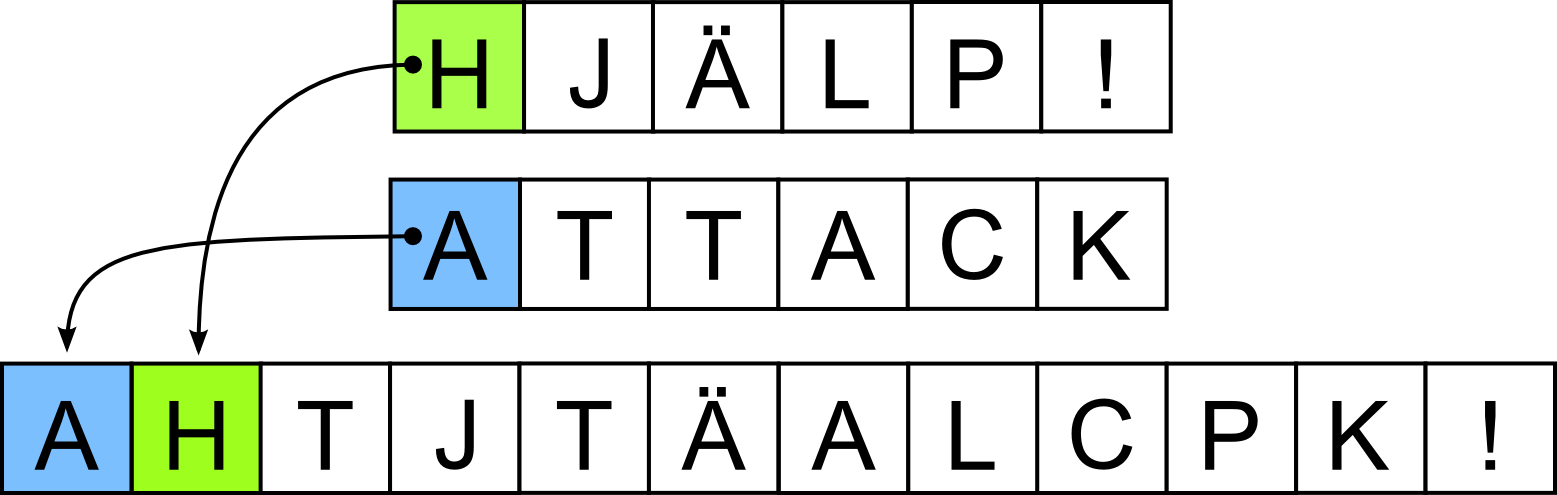
\includegraphics[width=\textwidth]{subst}

Ett hemligt meddelande på två rader sätts ihop till längre chiffertext.\newline
\end{center}

\noindent Ett tidigt exempel på teckensubstituering användes av Julius Caesar för att skicka meddelanden som var viktiga nog att klassas som militära. Metoden kallas för Caesarrullning och innebär att man substituerar bokstäverna med dem som ligger ett visst steg framåt i alfabetet. I den variant Caesar använde för att skicka meddelanden flyttades bokstäverna tre steg framåt, så att A blev D, B blev E och så vidare.\newline

\begin{center}
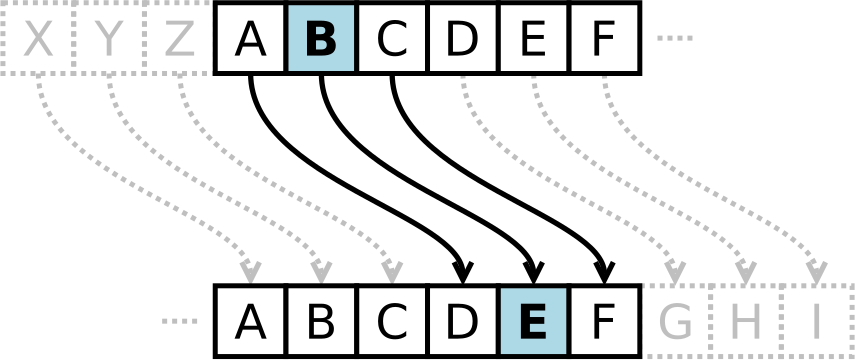
\includegraphics[width=\textwidth]{caesar}

Caesarrullning av alfabetet med 3 steg, samma nyckel som Caesar använde.\newline
\end{center}

\noindent Dessa kryptografiska systems säkerhet bygger dock på att man inte känner till hur meddelandet är dolt. Caesarrullning på det latinska alfabetet ger 26 möjliga nycklar, dvs lika många som antalet tecken. Att rulla 1 och 27 steg är identiskt då A byts ut mot B i båda fallen. Det svenska alfabetet hade istället givit 29 möjliga nycklar.

Hade Caesars fiender känt till denna krypteringsmetod och att den användes hade den inte givit någon riktig säkerhet. Antalet nycklar är tillräckligt få för att alla ska kunna testas. Intresset kommer att finnas, speciellt om det gäller militära hemligheter.

Låter man istället varje tecken ersättas med ett annat så att ett tecken representerar ett annat; A till B, B till G, Z till F,  får man \[26! = 403.291.461.126.605.635.584.000.000\] möjliga nycklar. Numret är så obegripligt stort att det blir orealistiskt att gå igenom alla möjliga nycklar.

Att knäcka kodsystem, \emph{kryptoanalys}, har också sin historia. Ett tidig arabiskt dokument från 800-talet beskriver svagheter i caesarrullning. Att omkoda på det här sättet tar inte bort språkets karaktär ur meddelandet utan byter endast ut de tecken som används. Svagheter kan ligga i ord som statistiskt sett används ofta, eller tecken. I det engelska språket till exempel är bokstaven \emph{e} statistiskt vanligare än andra. Används då en bokstav i chiffertexten oftare än andra, kan man anta att denna motsvarar bokstaven e. Taktiskt val av nycklar att testa mot gör att man statistiskt sett kan hitta den rätta nyckeln väldigt mycket snabbare.

Den tekniska utveckligen ledde till slut till att både kodning och avkodning gjordes mekaniskt. Ett välkänt exempel på detta är Enigma-masiknen som utvecklades i början av 1920-talet.

Enigma började snabbt användas av tyska militären. Den första framgångsrika kryptoanalysen av maskinen gjorde att Polen fick möjlighet att avkoda flera av de upptagna meddelanden i mitten av 30-talet. Maskinen användes dock fortfarande av Tyskland under andra världskriget. Själva maskinen hade, trots sina svagheter, inte knäckts så mycket som kan framställas. Det var endast tillsammans med andra faktorer, som misstag gjorda av operatörer, och att de allierade fick tag i både maskiner och kodböcker, som de allierade kunde avkoda knäckta meddelanden.

Numera sker däremot nästan all kryptering digitalt med hjälp av datorer och är betydligt mer komplex än tidigare.\newline

\section {Modern kryptering}

Modern kryptering utförs med hjälp av datorsystem och långa nycklar. I takt med datorsystemens utveckling har det blivit väldigt mycket enklare att knäcka svagare krypton. Text i sig är även av en sådan natur att informationen inte behöver vara fullständigt korrekt för att man ska tyda meddelandet. Datorer kan även använda sig av ordlistor för att försöka knäcka krypteringen. Känner du utöver det till en del av den okrypterade texten går det att återhämta en del av nyckeln.

Moderna krypteringssystem designas för att ha så få svagheter som möjligt. Till att börja med är själva nyckeln lång nog för att det skulle ta orimligt lång tid att gå igenom varje enskild nyckel. Numera medför minsta lilla ändring i nyckeln ett helt annat resultat efter avkodning. Det går inte att tyda en avkodning som gjorts med \emph{nästan} rätt nyckel. Små förändringar ger lavinartade konsekvenser. \newline

\begin{center}
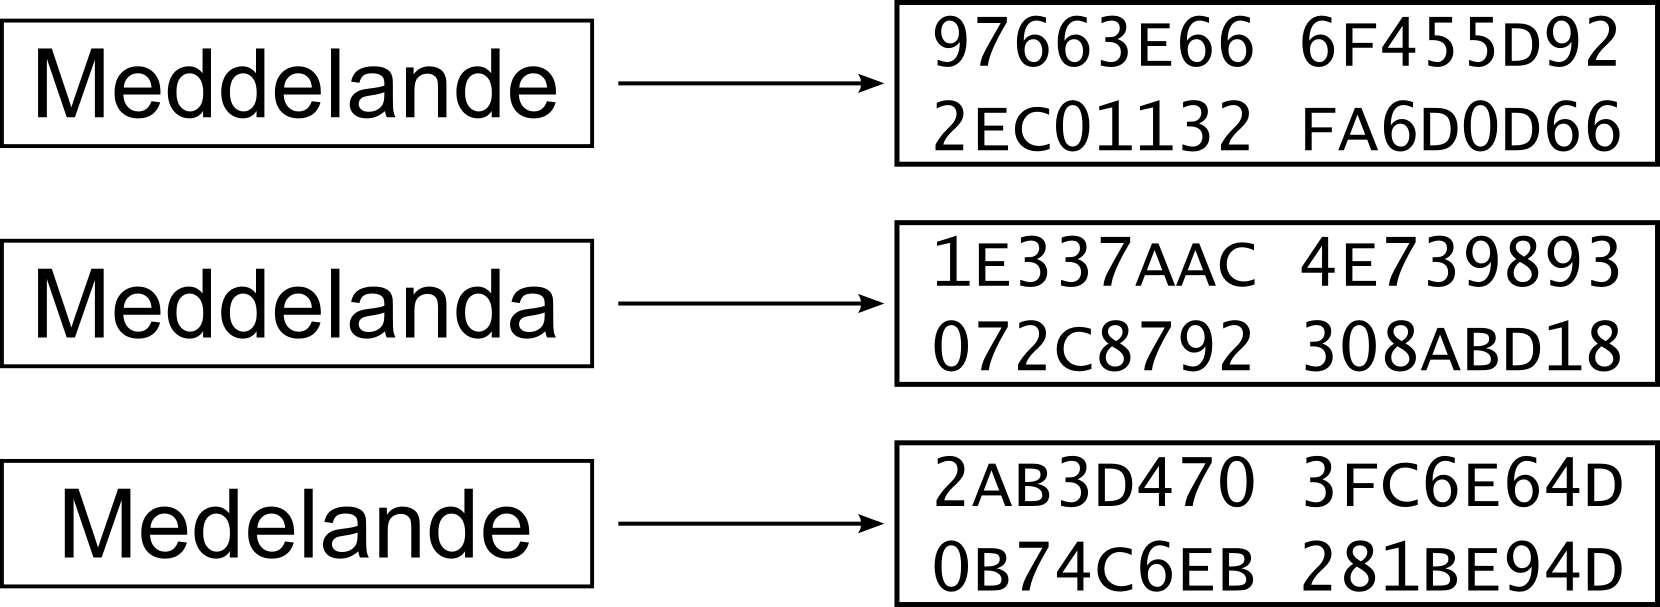
\includegraphics[width=\textwidth]{avalanche}

Kodning av olika meddelanden med hashfunktionen MD5. Bilden illustrerar hur minimala förändringar i texten ger lavinartade förändringar.
\end{center}

\noindent Det finns ett antal olika system som har sina för- och nackdelar. Vissa system är snabbare än andra, och vissa är mer invecklade och svårare att knäcka. Symmetrisk och assymetrisk kryptering som nämns nedanför har även olika användningsområden vilka kommer att visa sig.

	\subsection {Symmetrisk kryptering}
	
	Symmetrisk kryptering använder sig av en gemensam nyckel. Samma nyckel används för både kodning och avkodning av informationen. Den nyckel som säger att A ska bytas ut mot G i ett chiffer säger också helt enkelt att G ska bytas tillbaka till A när meddelandet ska tydas igen. Självklart är detta ett väldigt enkelt exempel.

		\subsubsection {Nyckelbestämmelse mellan två parter}

		Symmetrisk kryptering genomförs säkert även om en person avlyssnar all information som sänds över nätverket.

		Två datorer, A och B, kommunicerar med varandra. En tredje dator, C, förmedlar informationen som skickas mellan de båda parterna. Tillsammans kan då A och B bestämma en \emph{gemensam} nyckel, och både skicka och ta emot information krypterat från varandra \cite{applied-12-6}. C kan inte läsa av denna, eftersom C inte får reda på nyckeln.

		\subsubsection {Man in the Middle}

		Systemet för nyckelbestämmelse har dock en rejäl svaghet, och är inte säker från en medelpart som kan ändra informationen som skickas. Den är endast säker från direkt avlyssning. Varken A eller B kan försäkra sig om att det verkligen är A och B som de direkt pratar med. Fast de tror att de upprättat en säker anslutning med varandra kan den i själva verket ha upprättats tillsammans med någon annan.

		Mellanparten C förmedlar trafik mellan A och B. C förmedlar däremot under attacken inte bara trafik vid nyckelutbytet utan tar en mer aktiv roll. C uppger sig för att vara den andra parten åt båda hållen och bestämmer två separata nycklar med både A och B. A och B som tror att en säker anslutning är skapad börjar sedan skicka information. A kodar sitt \emph{meddelande} och skickar till C, som sedan avkodar meddelandet. C tar del av informationen, och eventuellt ändrar på den. Med nyckeln som bestämts mellan C och B krypteras informationen igen och skickas vidare till B. Eftersom ingen identitetsförsäkran gjorts har varken A eller B någon aning om vem de egentligen pratar med.\newline

\begin{center}
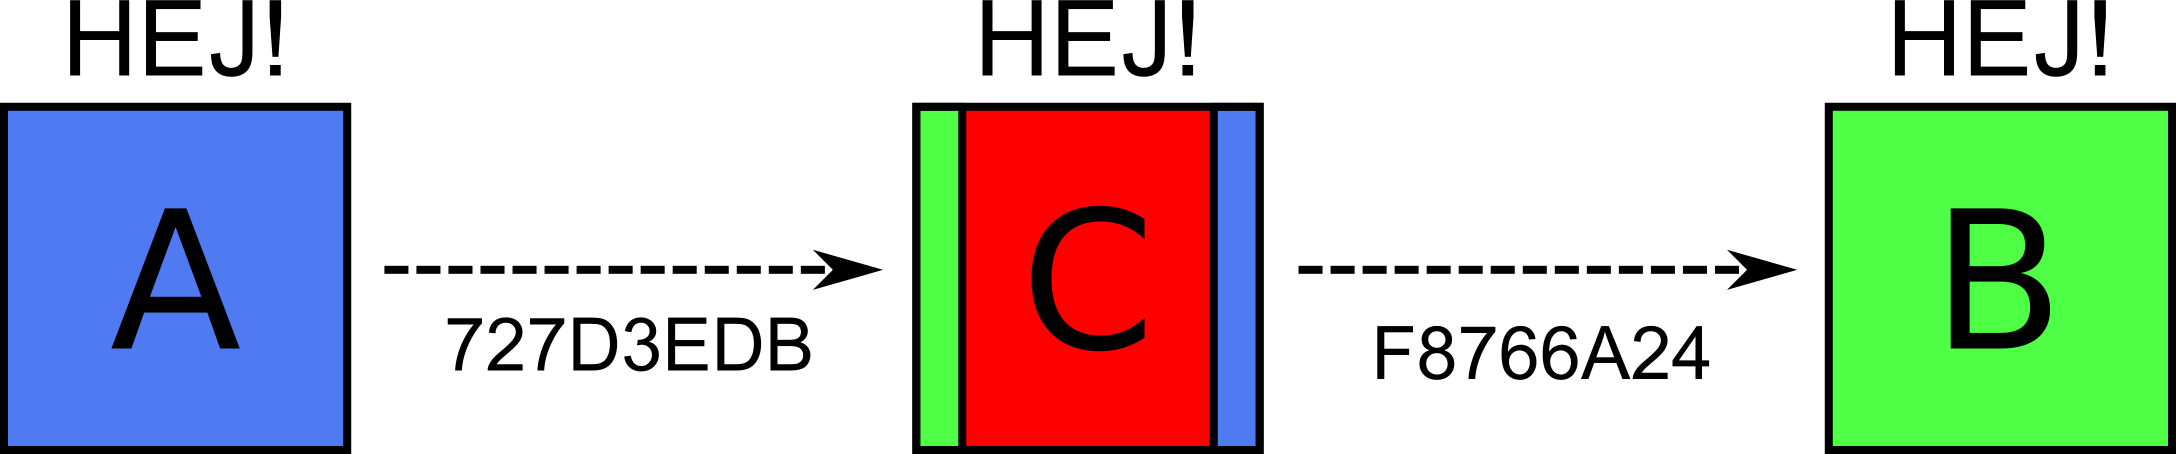
\includegraphics[width=\textwidth]{janus}

Man in the Middle-attack. Båda parterna tror att de pratar direkt med varandra, mellanparten tyder allt som sägs, med möjlighet att ändra meddelandet.\newline
\end{center}

	\subsection {Assymmetrisk kryptering}

	Assymmetrisk kryptering fungerar på ett annorlunda sätt. Varje part har två nycklar, varav en delas ut, och den andra hålls hemlig. Varje part känner till de andra parternas \emph{publika} nyckel och sin egen \emph{privata}.
	Den \emph{publika} nyckeln kan användas för att kryptera meddelanden som kan avkrypteras av mottagarens \emph{privata} nyckel. På samma sätt krävs den \emph{publika} nyckeln för att avkryptera meddelanden som krypteras av den \emph{privata}. Båda dessa relationer är väldigt viktiga. Den publika och privata nyckeln har i princip samma förhållande till varandra. Det är bara att man väljer ut en av dem att hålla hemlig. Den andra sprider man ut så väl som möjligt, då det förhindrar att andra trovärdigt kan sprida en falsk sådan nyckel \cite{applied-8-1}.

	Kryptering med den \emph{publika} nyckeln används för att skicka \emph{meddelanden} till ägaren av den \emph{privata} nyckeln. Då kan bara den som ska ta emot meddelandet dekryptera det. Här beror \emph{säkerheten} på hur hemlig den privata nyckeln är, annars kan den som tagit nyckeln även läsa meddelandet.

	Det går därför att skicka meddelanden som endast den avsedda mottagaren kan läsa. Kryptering åt andra hållet, då du krypterar med din egna \emph{privata} nyckel är också nödvändigt. Detta görs för att mottagaren ska kunna vara säker på att just du, ägaren av den privata nyckeln, har skickat meddelandet. Detta avkodas med din \emph{publika} nyckel. Här beror istället \emph{äktheten} på hur hemlig den privata nyckeln är, annars vet man inte vem som skickat meddelandet..

Problemet med äkthet av den privata och publika nyckelns faktiska ägare ligger kvar i teorin. Däremot måste denna relation endast etableras en gång. Spridning av den publika nyckeln sker heller inte på ett systematiskt sätt, utan bland annat via hemsidor, chat och på ett usb-minne. Genom dessa källor är det mycket svårt för en mellanpart att uppge sig för att vara den andra personen. Mellanparten inte kan förutse hur eller när nyckelutbytet utförs. En person kan inte i efterhand ta din identitet, så länge din privata nyckel hålls säker.

Assymmetrisk kryptering går även att använda för att distribuera symmetriska krypteringsnycklar \cite{applied-12-5}. Dessa kan sedan användas för symmetrisk kryptering mellan parterna.

\section {Användningsområden}

Kryptografi används som sagt för att skydda information. Kryptografi används både för att skydda lagrad information och se till att kommunikation hålls säker mellan två parter. Lagrad information kräver liksom all kryptering en nyckel för att tydas. Krypterad kommunikation ser dock även till att denna nyckel hålls hemlig vid överföring mellan två parter. Det är betydligt lättare att hålla lagrad information säker, då det inte krävs någon överföring av nyckel mellan parter där någon kan lyssna.

	\subsection {Lagring}

	Kryptering av data för lagring sker överallt, och dessa användningsområden är många.

	Lösenord på servrar brukar till exempel krypteras. Eftersom informationsläckor förekommer är detta en bra idé för att skydda användares lösenord. Dessa lösenord hålls säkra även om någon tar sig in på servern eller om det finns en läcka inom företaget. De är systematiskt säkra.

	Att kryptera lösenord är vettigt även på en lokal dator, så att de inte går att läsa av även om någon kommer åt hårddisken. Det kan även vara smart att kryptera e-legitimation, eftersom den legitimerande handlingen inte kräver mer identifiering än ett lösenord. Krypteras legitimationen med ytterligare ett krypto behövs det ännu en nyckel, ett lösenord för att använda legitimationen. Det blir alltså svårare att knäcka.

	Självklart finns det även annan information som vi håller personlig och inte vill visa alla. Det här kan vara allt från affärsidéer till webbläsarhistorik, brev och bilder eller annat känsligt.

	Man behöver inte ha något speciellt att dölja för att hålla post eller information personlig. Kryptering är ett effektivt sätt att hålla brev och information privat, även för datoranvändare.

		\subsubsection {Hårddiskkryptering}

		Ett enkelt sätt att få ett mer privat datoranvändande är att kryptera den hårddisk som används, eller en del av den. Detta gäller speciellt på bärbara datorer eller datorer med flera användare. Så fort hårddisken som används riskerar att kommas åt av andra kan det vara en bra idé att kryptera hårddisken.

		Alternativ till att kryptera hårddisken är att skapa en virtuell, krypterad sådan. Den virtuella hårddisken sparas som en fil på datorn. Den virtuella hårddisken går efter att lösenordet matats in att använda precis som en vanlig hårddisk.\\

		\emph{TrueCrypt är ett exempel på mjukvara som används för hårddiskkryptering. Programmet är gratis, har öppen källkod och går att ladda ner från \url{http://www.truecrypt.org/}.}

	\subsection {Kommunikation}

	Krypterad kommunikation har också väldigt många potentiella användningsområden.
	
	Mobiltelefonsamtal är till exempel krypterade för att de inte ska gå att avlyssna på plats. Likaså kan även information som filer och mail krypteras när de skickas för att undvika avlyssning.

		\subsubsection {E-mail}

		E-mail är ett extra känsligt användningsområde. I dessa sammanhang är okrypterad trafik farlig. E-mail som skickas kan vara väldigt personliga. Identifikationsprocessen försvinner också till viss del, då det går lättare att utge sig för att vara någon annan.

		Kryptering av mailtrafiken innebär att den som skickar ett brev kan försäkra sig om att det kommer fram oläst. Den som tar emot brevet kan försäkra sig om att den som skickade brevet verkligen är den den utger sig för.

		Spam kan använda sig av okrypterad trafik och utge sig för att vara ens arbetsgivare, kompis eller liknande. Om post vanligtvis inte skickas krypterad, så kommer den som får mailet inte att märka någon skillnad. Som tur är brukar däremot spam vara ganska lätt att upptäcka då dessa brev ofta är väldigt dåligt skrivna.

		Men säg att någon skulle skriva ett välskrivet personligt brev och utge sig för att vara någon annan. Om krypteringsnycklar inte används i vanliga fall kan det bli väldigt svårt att avgöra om brevet är riktigt eller inte.

		Eftersom mail liksom telefonsamtal kan innehålla väldigt personlig information kan det även vara viktigt att kunna skicka information som garanteras hållas personlig. Okrypterad information kan avläsas av alla mellanparter som kan lyssna på kommunikationen. Personlig mailkryptering hindrar därför t.o.m. mailservrars ägare -- KTH, arbetsgivare eller till exempel Google för Gmail-användare -- från att läsa av detta.\\

		\emph{GNU Privacy Guard (GnuPG) är ett gratis program för e-mail-kryptering som även har öppen källkod och går att ladda ner på \url{http://gnupg.org/}. Det finns även diverse plug-ins för att förenkla användandet med diverse e-mailklienter och webbläsare. Information om några av dessa går att finna på artikeln om GnuPG på Wikipedia: \url{http://en.wikipedia.org/wiki/GNU_Privacy_Guard}.}

		\subsubsection {Banktransaktioner}

		Vid bankärenden över Internet är det väldigt viktigt att kunna verifiera att den som loggar in verkligen är den person som denne uppger sig för att vara.

		Just eftersom bankärenden är så viktiga brukar krypteringen här vara extra stark. Ett certifikat från en källa som anses säker brukar därför utfärdas. Denna garanterar att den privata nyckeln som utfärdas tillhör rätt ägare. På så sätt upprättas en säker anslutning mellan kunden och banken.

		Det är viktigt att förstå att kryptografin i sig inte är den enda svagheten i detta sammanhang. För att komma åt ett konto försöker man istället få tag på kort och koder på annat sätt. Detta inkluderar bl.a. att läsa av magnetremsor och sätta upp kameror vid bankomater.

		En annan svaghet i dessa sammanhang är att någon kan övervaka och använda ens dator. Får man tag på eventuella lösenord bland annat går det att kringgå all säkerhet som krypteringen innebär. Certifikat brukar därför kompletteras med lösenord som genereras eller levereras på andra sätt. Exempel på detta är bankdosor som används med ett speciellt kort för att generera en kod som matas in. En kod kan även levereras till exempel med rekommenderat brev eller via mobiltelefon.

\section {Svagheter i krypton}

Kryptoanalys av många, framför allt äldre, krypton har medfört att man lyckats knäcka flera krypton på kort tid. Principen för detta är följande: Om ett steg i kryptot som tar lång tid att beräkna går att ersätta med ett snabbt och mindre komplext steg kommer detta att kräva färre sökningar än vad ett test mot \emph{alla} nycklar hade krävt. Det kommer därför gå att räkna ut på kortare tid, och eventuellt närma sig genomförbart.

	Säg att ett tal ska multipliceras med ett annat och sedan multipliceras igen med ett tredje. Det går då att ersätta båda multiplikationer med \emph{en} enskild multiplikation. Detta skulle istället ta halva tiden att beräkna. Dessutom skulle man slippa testa att multiplicera både först med 2, sedan med 3, och först med 3 och sedan med 2. Detta skulle ersättas helt av att multiplicera med 6. Detta leder till att man behöver göra färre sökningar.

En annan säkerhetsbrist är att antalet möjliga nycklar helt enkelt är för få. Då kommer det vara möjligt att gå igenom alla nycklar inom rimlig tid.

Ett exempel på detta var den tidigare krypteringsstandarden DES, ``Data Encryption Standard'' som utvecklades av IBM 1974 och togs upp som en standard 1977 just eftersom den ansågs vara stark, och man hade inte hittat några stora svagheter i kryptot \cite{ibm}. DES svaghet ligger i den korta nyckel som används. Den nyckel som används med DES är endast 56 bitar lång, vilket ger \[2^{56}=72\ 057\ 594\ 037\ 927\ 936\] nycklar. Trots att detta kan verka vara väldigt många nycklar visade det sig inte vara tillräckligt.

The Electronic Frontier Foundation byggde 1998 en maskin för att söka efter en nyckel. Ingen speciell kryptoanalys användes, utan man gjorde helt enkelt en sökning efter nyckeln. Efter att ha gått igenom en fjärdedel av alla nycklar hittades nyckeln. Detta tog 56 timmar totalt, vilket betyder att alla nycklar skulle ta 4 dagar och 8 timmar \cite{eff}. DES visade sig alltså vara väldigt osäker.

	\subsection {Kombinationer av krypto}

	För att undvika olika svagheters påverkan kan man kombinera flera olika krypton. Dessa får då möjlighet att täcka över varandras svagheter. Principen är enkel. Finner man en svaghet i kryptot A, som gör att A i sig blir osäkert, kommer säkerheten i B fortfarande finnas kvar. Båda måste brytas rejält för att informationen ska bli osäker. Ett försök att bryta kryptot genom att använda alla nycklar kommer att vara betydligt svårare att genomföra. Man behöver för varje prövad nyckel till A testa varje nyckel som finns möjlig för B. Antalet kombinationer som man behöver gå igenom för att knäcka kryptot ökar därför drastiskt.

		\subsubsection {Triple-DES}

		Eftersom DES svaghet låg i nyckelns längd skapades Triple-DES. DES kan ses som en förlängning av DES-standarden. Säg att du väljer tre nycklar, A, B och C. Den okrypterade informationen skickas sedan igenom DES tre gånger, med de separata nycklarna var för sig. Nyckeln som behövs för att avkoda informationen som kom ur Triple-DES kommer att vara tre gånger så lång som originalnyckeln, och därför långt ifrån lika sårbar  som enkla DES för en sådan s.k. \emph{brute force}-attack. DES använder som tidigare nämnt en nyckel på 56 bitar, vilket ger $2^{56}$ möjliga nycklar. Triple-DES använder istället tre sådana nycklar, vilket ger en nyckellängd på 168 bitar. Alltså kommer en genomgång av alla nycklar för Triple-DES att ta $2^{112}$ gånger längre tid. Om originalet tar ens en minut att knäcka, vilket är långt under den tidigare knäckningen, så kommer det att vara omöjligt att söka efter nycklar på samma sätt som användes vid knäckningen av DES.

		\subsubsection {Olika krypton}
		
		Det finns däremot en fördel med att blanda \emph{olika} krypton annat än att få en längre nyckel. Nyckeln är nämligen endast viktig om den behövs för att knäcka kryptot. Om ett kryptos design upptäcks vara väldigt trasig kan egentligen inte en längre nyckel rädda dig från problemet. Risken att två \emph{olika} krypton skulle ha väldigt stora säkerhetsläckor är däremot betydligt mindre. Det kan därför vara smart att kombinera flera krypton.

\section {Förslag till åtgärder}

Just eftersom det ständigt upptäcks läckor i flera, framför allt äldre, kryptografiska system är det viktigt att hålla sig uppdaterad. Det är väldigt riskfyllt att fortsätta använda lättknäckta krypteringssystem. Att kryptering över huvud taget finns hjälper till viss del att hålla de flesta borta, men däremot behöver äldre krypteringssystem inte ge någon \emph{riktig} säkerhet.

Så fort ett krypto knäcks bör informationen ses som oskyddad i den mån att alla som \emph{verkligen} vill komma åt den kan komma åt den. Det symboliska skyddet finns självklart fortfarande kvar. Har den krypterade informationen inte läckt än kan säkerheten däremot uppgraderas genom att byta kryptering på det som redan är lagrat. Det är ändå en bra idé att byta kryptering för framtida information som ska lagras.

Uppsatsen har som tidigare nämnts ämnat ta upp flera användningsområden. Viktigast att tänka på för läsaren anses vara e-mail- och hårddiskkryptering. Att använda sig av både och är väldigt enkelt, detta rekommenderas om man vill hålla sina brev och filer privata som tidigare beskrivet. Dessa användningsområden behöver slutanvändaren själv tänka på, till skillnad från banktransaktioner där systemen är byggda för att vara säkra.

\newpage

\begin{thebibliography}{99}

\bibitem{cqchist} Centre for Quantum Computation, University of Cambridge. \emph{History of Cryptography}.\\
URL: \url{http://cam.qubit.org/articles/crypto/intro.php} (Hämtad 2008-11-22)

\bibitem{applied} Menezes, A., van Oorschot, P. och Vanstone, S. (2001). \emph{Handbook of Applied Cryptography}\\
URL: \url{http://www.cacr.math.uwaterloo.ca/hac/}, ISBN: 0-8493-8523-7.

\bibitem{applied-8-1} \emph{Public-Key Cryptography, Introduction} \\
Handbook of Applied Cryptography, del 8.1, s. 283.

\bibitem{applied-12-6} \emph{Key Establishment Protocols, Key agreement based on asymmetric techniques} \\
Handbook of Applied Cryptography, del 12.6, s. 515-524.

\bibitem{applied-12-5} \emph{Key Establishment Protocols, Key transport based on public-key encryption} \\
Handbook of Applied Cryptography, del 12.6, s. 515.

\bibitem{ibm} Coppersmith, Dan. \emph{The Data Encryption Standard and its strength against attacks} \\
IBM Journal ofo Research and Development, 38(3), s. 243-250.

\bibitem{eff} The Electronic Frontier Foundation, \emph{Frequently Asked Questions (FAQ) About the Electronic Frontier Foundation's "DES Cracker" Machine} \\
URL: \url{http://w2.eff.org/Privacy/Crypto/Crypto_misc/DESCracker/HTML/19980716_eff_des_faq.html} (1998-07-11).

\end{thebibliography}

\end{document}
